\documentclass[letterpaper,11pt]{article}
\usepackage[hmargin=0.5in,vmargin=1in]{geometry}
\usepackage[english]{babel}
\usepackage[utf8]{inputenc}
\usepackage{amsmath,amsthm}
\usepackage{algorithmic}
\usepackage{algorithm}
\usepackage{enumerate}  
\usepackage{subfig}
\usepackage{amssymb}
\usepackage{mathtools}
\usepackage{graphicx,color,xcolor}
\usepackage{bm}
\usepackage{tcolorbox}
\usepackage{hyperref}
\usepackage{listings}
\usepackage{graphicx}

\definecolor{deepblue}{rgb}{0,0,0.5}
\definecolor{deepred}{rgb}{0.6,0,0}
\definecolor{deepgreen}{rgb}{0,0.5,0}

\definecolor{codegreen}{rgb}{0,0.6,0}
\definecolor{codegray}{rgb}{0.5,0.5,0.5}
\definecolor{codepurple}{rgb}{0.58,0,0.82}
\definecolor{backcolour}{rgb}{0.95,0.95,0.92}

\lstdefinestyle{mystyle}{
	%	backgroundcolor=\color{backcolour},   
	commentstyle=\color{codepurple},
	keywordstyle=\color{green},
	numberstyle=\tiny\color{codegray},
	stringstyle=\color{red},
	%	basicstyle=\ttfamily\footnotesize,
	breakatwhitespace=false,         
	breaklines=true,                 
	captionpos=b,                    
	keepspaces=true,                 
	numbers=left,                    
	numbersep=5pt,                  
	showspaces=false,                
	showstringspaces=false,
	showtabs=false,                  
	otherkeywords={vector, string},
	escapechar={|}, 
	tabsize=2
}

\lstset{style=mystyle}
\hypersetup{
	colorlinks=true,
	linkcolor=blue,
	filecolor=magenta,      
	urlcolor=cyan,
}

\title{{\bf GHS Implementation Report}}
\author{2017CS50405 Dhananjay Kajla \\ 2017CS50421 Vijay Kumar Meena}
\date{12$^{th}$ April 2021}

\begin{document}
	
	
	
	\maketitle
	
	\tableofcontents
	
	\section{Introduction to the GHS Algorithm}
	
	The GHS Algorithm (named after it's authors Gallager, Humblet and Spira) was first published in a 1983 \href{https://dl.acm.org/doi/abs/10.1145/357195.357200}{paper}. It gives an asynchronous distributed algorithm that runs identically on each node and in due time, each node learns which of it's incident edges belong in the minimum spanning tree. \\
	
 	
 	The algorithm essentially works by creating, expanding and merging fragments of the graph. These fragments are guaranteed to be a part of the final MST of the complete graph. \\
 	
 	Each node can be in one of 3 states : {\sc Sleep}, {\sc Find} and {\sc Found}. \\
 	
 	For a node, the edge between every neighbor can be in one of 3 states : {\sc Basic}, {\sc branch} and {\sc reject}. \\ 
 	
 	In basic state represents an edge that is yet to be tested for its presence in the MST. An edge in state branch represents an edge that is known to be in the final MST. And an edge in reject state has been rejected and cannot be a part of the MST. \\
 	
 	At the start of the algorithm, all nodes are in state {\sc Sleep}, they are either woken up by a message, or they wake up spontaneously. For getting the best bound on messages, we shall assume that all nodes are woken up simultaneously at the start. \\
 	
 	After that each node can either be in state {\sc Find} where it is looking for new edges for MST or it can be in state {\sc Found} when it's passive. \\
 	
 	Each node has a {\sc Level} and a {\sc Name} which is representative of it's fragment. Two fragments combine when either the node with smaller requests a connection to the larger or when two nodes with same level combine and form a node with level incremented by one. The first case is called the LT rule of merging, and the second case is the EQ rule. \\
 	explain
 	The nodes communicate through the following types of messages : 
 	\begin{itemize}
 		\item {\sc Connect} : Request for merging the two nodes.
 		\item {\sc Initiate} : Communicates new fragment level and identity to the neighbors
 		\item {\sc Test} : Tests to check whether an edge belongs to the MST
 		\item {\sc Accept} : Communicates to the neighbor that the received edge tested is accepted into the MST
 		\item {\sc Reject} : Communicates to the neighbor that the received edge cannot possibly be in the MST
 		\item {\sc Report} : Reports the best weight outgoing fragment for each node 
 		\item {\sc ChangeRoot} : The root node of the fragment is shifted to the node with the minimal outgoing edge
 	\end{itemize}
 
 	Under the assumption of initial awakening of all the nodes, GHS Algorithm guarantees the number of messages sent to be $< 2\cdot E + 5 \cdot N \cdot \log_2(N)$. We shall see more about this in our experiments \\
	
	We shall see the algorithm itself in next section :
	
	\section{Implementation Details}
	
	We have implemented a multi-threaded parallel implementation of the GHS Algorithm. Each node of the GHS is given a single thread in the implementation. \\ 
	
	In this section, we shall outline the two parts of our implementation : 
	\begin{enumerate}
		\item Inter-Thread Communication 
		\item GHS Algorithm at each node
		\item Main Function that runs thread
	\end{enumerate}
	
	\subsection{Inter-Thread Communication}
	
	\subsubsection{Messages}
	
	The messages sent by the threads(nodes) are dynamic arrays of strings. \\
	
	We have created a message class to standardize all messages : 
	\begin{lstlisting}[language=C++, caption = Message Class]
		class Message
		{
		private:
			std::vector<std::string> msg; //!< message content
		public:
			|\color{blue}Message|(std::vector<std::string> m) //!< Initiates a message
			{
				msg = m;
			}
			std::vector<std::string> |\color{blue}getMessage|() //!< returns the message
			{
				return msg;
			}
		};
	\end{lstlisting}
	
	\newpage
	
	For the ease of sending messages, we have created the a helper function {\sc msgCreater}() : 
	
	
	\begin{lstlisting}[language=C++, caption = msgCreater]
		
		Message *GHSNode::|\color{blue}msgCreater|(std::vector<std::string> msg)
		{
			std::vector<std::string> m;
			m.|\color{cyan}push\_back|(std::|\color{cyan}to\_string|(nodeid));
			
			for(auto it : msg)
			{
				m.|\color{cyan}push\_back|(it);
			}
			
			Message *mg = new Message(m);
			return mg;
		}
	\end{lstlisting}
	
	\bigskip
	
	This dynamic array has the structure : \{sender\_id, Message type, Parameter1, Parameter2, ...\} \\
	
	Here is an example of message sending ({\sc sendMessage}() will be explained later) : 
	
	
	\begin{lstlisting}[language=C++, caption = sendMessage Sample]
		m.|\color{cyan}push\_back|("initiate"); //!< Initiate()
		m.|\color{cyan}push\_back|(std::|\color{cyan}to\_string|(LN)); //!< LN
		m.|\color{cyan}push\_back|(FN); //!< FN
		m.|\color{cyan}push\_back|(SN); //!< SN
		
		sendMessage(j, msgCreater(m)); //!< send Initiate(LN, FN, SN) on edge j 
	\end{lstlisting}
	
	\subsubsection{Queues}
	
	To handle simultaneous messages, we have defined a thread safe data structure {\sc Queue} built upon the std::queue provided by the Standard Template Library of C++ : 
	
	\begin{lstlisting}[language=C++, caption = Queue]
	class Queue
	{
		private:
		std::|\color{green}mutex| mut; //!< mutex lock for thread safety
		std::|\color{green}queue|<Message *> q; //!< Message queue
		int queueid; //!< Id of the node to which this queue belongs
		public:
		|\color{blue}Queue|()
		{
			queueid = -1; //!< Initialized as bad node
		}
		|\color{blue}Queue|(int qid)
		{
			queueid = qid; //!< ID of the queue
		}
		int |\color{blue}getqueueid|()
		{
			return queueid; //!< returns id for the node which owns this queue
		}
		void |\color{blue}push|(Message *m)
		{
			mut.|\color{cyan}lock|(); //!< Puts the lock in place
			q.|\color{cyan}push|(m); //!< This push operation is atomic
			mut.|\color{cyan}unlock|(); //!< Unlocks the queue
		}
		Message *|\color{blue}front|()
		{
			mut.|\color{cyan}lock|(); //!< Puts the lock in place
			if(q.|\color{cyan}size|() == 0)
			{
				mut.|\color{cyan}unlock|(); //!< Unlocks the queue
				return NULL; //!< Returns NULL if queue is empty
			}
			Message *temp = q.|\color{cyan}front|(); //!< This front operation is atomic
			mut.|\color{cyan}unlock|(); //!< Unlocks the queue
			return temp;
		}
		Message *|\color{blue}pop|()
		{
			mut.|\color{cyan}lock|(); //!< Puts the lock in place
			int temp = q.|\color{cyan}size|(); //!< Temporary variable to store queue size
			if(temp == 0)
			{
				mut.|\color{cyan}unlock|(); //!< Unlocks the queue
				return NULL; //!< Returns NULL if queue is empty
			}
			Message *tmp = q.|\color{cyan}front|(); //!< Temporary variable to store the front of queue
			q.|\color{cyan}pop|(); //!< Pops the queue
			if((int)q.|\color{cyan}size|() != temp - 1) //!< Pop should change the size of queue by 1
			{
				std::cerr << "QUEUE Error" << std::endl; 
				|\color{cyan}exit|(1);
			}
			mut.|\color{cyan}unlock|(); //!< Unlocks the queue
			return tmp;
		}
		bool |\color{blue}empty|()
		{
			mut.|\color{cyan}lock|(); //!< Puts the lock in place
			int temp = q.|\color{cyan}size|(); //!< Temporary variable for queue size
			mut.|\color{cyan}unlock|(); //!< Unlocks the queue
			return (temp == 0); //!< Returns if queue is empty
		}
		int |\color{blue}getQueueSize|()
		{
			mut.|\color{cyan}lock|(); //!< Puts the lock in place
			int temp = q.|\color{cyan}size|(); //!< Size of queue
			mut.|\color{cyan}unlock|(); //!< Unlocks the queue 
			return temp; //!< returns size of queue
		}
	};
	\end{lstlisting}
	
	Each thread(node) gets it's own Queue instance, which is instantiated in the Network class. A thread which of the queue has all the operations available to it whereas a non-owner thread can only {\color{cyan}push} to the queue. \\
	
	Each node (i.e. each Instance of the GHSNode class) is provided with a pointer to it's queue at it's instantiation. The pointer to other node's queue can be taken from the Network class which we describe next.
		
	\subsubsection{Network}
	
	To send and receive messages from different nodes, we have a defined an internet of sorts for the threads. This is the {\sc Network} class : \\
	
	\begin{lstlisting}[language=C++, caption= Network]
		class Network
		{
		private:
			std::|\color{green}unordered\_map|<int, Queue *> msg_queues; //!< Network queues
		public:
			|\color{blue}Network|(std::|\color{green}vector|<int> nodes) //!< Network Constructor 
			{
				for(auto it : nodes)
				{
					Queue *q = new Queue(it); //!< Initiates a new queue
					msg_queues[it] = q; //!< Initializes the hashmap
				}
			}
			Queue *|\color{blue}getQueue|(int i) //!< Get's the ith queue
			{
				if(msg_queues.|\color{cyan}find|(i) == msg_queues.|\color{cyan}end|())
				{
					std::cerr << "BAD network Request" << std::|\color{cyan}endl|;
				}
				return msg_queues[i]; //!< Returns the pointer to ith queue
			}
		}
		;
	\end{lstlisting}
	
	The {\sc Network} class is instantiated only once, and each node keeps a pointer to the single instance.  
	
	\subsubsection{IsComplete}
	
	{\sc IsComplete} is a class which we have defined to trigger the end of the algorithm. This is a thread join of sorts. Once this is complete we shutdown all nodes and ask them for the part of MST that they posses. \\
	
	This class is instantiated only once and every node possesses a pointer to this instance so that any node can give out the halt signal.
	
	\begin{lstlisting}[language=C++, caption= IsComplete]
		struct IsComplete
		{
			bool complete; //!< If set true, the threads exit
			|\color{blue}IsComplete|() //!< Constructor that sets the default value false
			{
				complete = false; 
			}
		};
		
	\end{lstlisting}
	
	\subsubsection{GHS Algorithm Constructor}
	
	To show what we pass to each node initially, we shall list out the constructor for the GHSNode : 
	
	\begin{lstlisting}[language=C++, caption= GHSNode constructor]
		GHSNode::GHSNode(int nid, std::|\color{green}unordered\_map|<int, int> &neighbors, Network *net, IsComplete *iscom)
		{
			this->nodeid = nid;
			this->nbd = neighbors;
			this->network = net;
			this->SN = "sleep";
			this->isc = iscom;
			this->nodequeue = net->getQueue(nid);
		}
	\end{lstlisting}

	As we can see, each node receives the pointer to it's queue and the pointer to the network along with the IsComplete instance.  \\
	
	\subsubsection{Sending and Receiving messages}
	
	Now to summarize the thread messaging, let us give the code snippets for the {\sc sendMessage}() and {\sc receiveMessage}() methods : 
	
	\begin{lstlisting}[language=C++, caption= sendMessage]
		void GHSNode::|\color{blue}sendMessage|(int dest, Message *m)
		{
			Queue *q = network->getQueue(dest);
			q->|\color{cyan}push|(m);
		}
	\end{lstlisting}
	
	\begin{lstlisting}[language=C++, caption= receiveMessage]
		bool GHSNode::recieveMessage()
		{
			msg = nodequeue->|\color{cyan}pop|();
			return (msg != NULL);
		}
	\end{lstlisting}

	This completes our summary of thread communication 
	
	\subsection{GHS Algorithm implementation at each node}
	
	Each GHSNode has the following state variables :  \\  
	
	\begin{tabular}{|c|c|c|}
		\hline
		\bf{Variable Name} & \bf{Variable Title} & \bf{Range of the variable} \\
		\hline 
		NodeId & Id of the node &  $\mathbb{N}$ \\
		\hline
		SN & State of the node & ["sleep" , "find" , "found"] \\
		\hline
		FN & Name of the node & - \\
		\hline
		LN & Level of the node & $\mathbb{N}$ \\
		\hline
		nbd & Adjacency list & $\{key : value\} \text{ key } \in \mathbb{N} \text{, } \text{value} \in \mathbb{N} $ \\
		\hline
		SE & State of edges & ["baisc", "branch", "reject"] \\
		\hline 
		best-edge & Currently the minimum weight outgoing edge & $\mathbb{N}$ \\
		\hline
		best-weight & Current best outgoing weight & $\mathbb{N}$ \\
		\hline 
		test-edge & Edge currently being tested & $\mathbb{N}$ \\
		\hline 
		in-branch & Parent node of sorts & $\mathbb{N}$ \\
		\hline 
		find-count & number of MST Edges found & $\mathbb{N}$ \\
		\hline 
	\end{tabular}

	\bigskip 
	
	The following types of messages can be sent : \\
	
	\bigskip
	
	\begin{tabular}{|c|c|c|}
	\hline
	\bf{Message Type} & \bf{Description} & \bf{Parameters} \\
	\hline
	Connect & Request for merging the two nodes & Level \\
	\hline
	Initiate & Communicates new fragment level and identity to the neighbors & Level, Name, State \\
	\hline
 	Test & Tests to check whether an edge belongs to the MST & Level, Name \\
 	\hline
	Accept & Received test edge is accepted into the MST & - \\
	\hline
	Reject & Received test edge cannot possibly be in the MST & - \\
	\hline
	Report & Reports the best weight outgoing fragment for each node & best weight \\ 
	\hline
	ChangeRoot & Start Changing root of fragment  &  - \\
	\hline
	\end{tabular}

	\medskip
	
	We will now list the 12 Algorithms as mentioned in the original GHS \href{https://dl.acm.org/doi/abs/10.1145/357195.357200}{paper} and our implementation for the same. \\
	
	These are long pseudocodes and codes. If required one can skip to the \hyperlink{s2d4}{next} subsection on thread\_runner.
	
	\subsubsection{Algorithm 1}
	Spontaneous awakening at each node at the starting instant. {\sc run}() is the function that the thread starts. 
	
	\begin{lstlisting}[language=C++, caption= run]
		void GHSNode::run()
		{
			wakeup();
			runner();
		}
	\end{lstlisting}
	
	\subsubsection{Algorithm 2}
	Pseudocode : \\
	
	\begin{tcolorbox}
	wakeup()
	\begin{algorithmic}
		\STATE \textbf{begin}
		\STATE let $m$ be adjacent edge of minimum weight 
		\STATE $SE(m) \leftarrow Branch$; 
		\STATE $LN \leftarrow 0$;
		\STATE $SN \leftarrow Found$;
		\STATE $Find-count \leftarrow 0$;
		\STATE {\bf{send}} $Connect(0)$ on edge $m$
	\end{algorithmic}
	\end{tcolorbox}

	\bigskip 
	
	Implementation : 
	
	
	\begin{lstlisting}[language=C++, caption= wakeup]
	void GHSNode::|\color{blue}wakeup|()
	{
		if(nbd.|\color{cyan}empty|())
		{
			isc->complete = true;
		}
		
		for(auto it : nbd)
		{
			SE[it.first] = "basic";
			basic.|\color{cyan}insert|(std::|\color{green}make\_pair|(it.second, it.first));
		}
		
		int m = |\color{cyan}findMinEdge|(); // let m be adjacent edge of minimum weight;
		|\color{cyan}changestat|(m, "branch"); //!< SE(m) <- Branch
		LN = 0; //!< LN <- 0
		SN = "found"; //!< SN <- Found
		find_count = 0; //!< Find-count <- 0
		std::vector<std::string> st;
		st.|\color{cyan}push\_back|("connect");
		st.|\color{cyan}push\_back|(std::|\color{cyan}to\_string|(LN));
		|\color{cyan}sendMessage|(m, |\color{cyan}msgCreater|(st)); //!< send Connect(0) on edge m
	}
	\end{lstlisting}
	
	\subsubsection{Algorithm 3}
	Pseudocode : \\
	
	\begin{tcolorbox}
		Response to $Connect(L)$ on edge $j$
		\begin{algorithmic}
			\STATE \textbf{begin} {\bf if} $SN = Sleeping$ {\bf then execute procedure }wakeup; \\
			{\quad \qquad  \bf if } $L < LN$ \\
			{\quad \qquad  \bf then begin } $SE(j) \leftarrow Branch$; \\
			{\qquad \qquad \qquad \qquad \bf send } $Initiate(LN, FN, SN)$ on edge $j$ \\
			{\qquad \qquad \qquad \qquad \bf if } $SN = Find$ {\bf then} \\
			{\qquad \qquad \qquad \qquad \quad } $find\_count \leftarrow find\_count + 1$ \\
			{\qquad \qquad  \qquad \bf end } \\
			{\quad \qquad  \bf else if } $SE(j) = Basic$ \\
			{\qquad \qquad \qquad \bf then } place received message on end of queue \\
			{\qquad \qquad \qquad \bf else send} $Initiate(LN+1, w(j), Find)$ on edge $j$ \\
			{\bf end}
		\end{algorithmic}
	\end{tcolorbox}
	
	\bigskip 
	
	Implementation : 
	
	
	\begin{lstlisting}[language=C++, caption= handleConnect()]
		void GHSNode::|\color{blue}handleConnect|()
		{
			std::vector<std::string> mg = msg->getMessage();
			int j = std::|\color{green}stoi|(mg[0]); //!< edge j
			int L = std::|\color{green}stoi|(mg[2]); //!< L
			if(SN == "sleep")      //!< if SN = Sleeping 
			{
				|\color{cyan}wakeup|(); //!< execute procedure wakeup
			}
			if(L < LN) //!< If L < LN
			{
				|\color{cyan}changestat|(j, "branch");
				
				std::vector<std::string> m; 
				m.|\color{cyan}push\_back|("initiate"); //!< Initiate()
				m.|\color{cyan}push\_back|(std::|\color{cyan}to\_string|(LN)); //!< LN
				m.|\color{cyan}push\_back|(FN); //!< FN
				m.|\color{cyan}push\_back|(SN); //!< SN
				
				|\color{cyan}sendMessage|(j, |\color{cyan}msgCreater|(m)); //!< send Initiate(LN, FN, SN) on edge j 
				
				if(SN == "find") //!< if SN = Find then
				{
					find_count++; //!< find-count <- find-count +1
				}
				
				|\color{cyan}free|(msg);
				msg = NULL;
			}
			else if(SE[j] == "basic") //!< else if SE(j) = Basic
			{
				|\color{cyan}sendMessage|(nodeid, msg); //!< place receieved message on end of queue
			}
			else
			{
				std::vector<std::string> st; 
				st.|\color{cyan}push\_back|("initiate"); //!< Initiate()
				st.|\color{cyan}push\_back|(std::|\color{cyan}to\_string|(LN+1)); //!< LN +1
				st.|\color{cyan}push\_back|(std::|\color{cyan}to\_string|(nbd[j]));//!< w(j)
				st.|\color{cyan}push\_back|("find");//!< Find
				|\color{cyan}sendMessage|(j, msgCreater(st)); //! send Initiate(LN+1, w(j), Find) on edge j
				|\color{cyan}free|(msg);
				msg = NULL;
			}
		}
	\end{lstlisting}
	
	\newpage
	
	\subsubsection{Algorithm 4}
	Pseudocode : \\
	
	\begin{tcolorbox}
		Response to $Initiate(L, F, S)$ on edge $j$
		\begin{algorithmic}
			\STATE \textbf{begin} $LN \leftarrow L; FN \leftarrow F;SN \leftarrow S; in\_branch \leftarrow j$; \\
			{\quad \qquad  \bf } $best\_edge \leftarrow nil; best\_wt \leftarrow \infty$; \\
			{\quad \qquad  \bf for all } $i \neq j$ such that $SE(i) = Branch$ \\
			{\qquad \qquad \quad \bf do begin send} $Initiate(L, F, S)$ on edge $i$; \\
			{\qquad \qquad \qquad \qquad \quad \bf if } $S = Find$ {\bf then} $find\_count \leftarrow find\_count + 1$; \\
			{\qquad \qquad  \qquad \quad \bf end } \\
			{\quad \qquad  \bf if } $S = Find$ {\bf then execute procedure} $test$\\
			{\bf end}
		\end{algorithmic}
	\end{tcolorbox}
	
	\bigskip 
	
	Implementation : 
	
	
	\begin{lstlisting}[language=C++, caption= handleInitiate()]
		void GHSNode::|\color{blue}handleInitiate|()
		{
			std::vector<std::string> mg = msg->getMessage();
			int j = |\color{green}stoi|(mg[0]); //!< edge j
			int L = |\color{green}stoi|(mg[2]); //!< L
			std::string F = mg[3]; //!< F
			std::string S = mg[4]; //!< S
			LN = L; //!< LN <- L
			FN = F; //!< FN <- F
			SN = S; //!< SN <- S
			in_branch = j; //!< in-branch <- j
			best_edge = -1; //!< best-edge <- nil
			best_weight = INF; //!< best-wt <- infinity
			for(auto it : branch) //!< forall
			{
				if(it.second == j)
				{
					continue;
				}//!< i != j and SE(i) = branch
				std::vector<std::string> st; 
				st.|\color{cyan}push\_back|("initiate"); //!< Initiate()
				st.|\color{cyan}push\_back|(std::|\color{cyan}to\_string|(L)); //!< L
				st.|\color{cyan}push\_back|(F); //!< F
				st.|\color{cyan}push\_back|(S); //!< S
				|\color{cyan}sendMessage|(it.second, |\color{cyan}msgCreater|(st)); //!< send Initiate(L, F, S) on edge i
				if(S == "find") //!< if S = Find 
				{
					find_count++; //!< find-count <- find-count + 1
				}
			}
			if(S == "find") //!< if S = Find
			{
				|\color{cyan}test|(); //!< execute procedure test
			}
			|\color{cyan}free|(msg);
			msg = NULL;
		}
	\end{lstlisting}
	
	
	\subsubsection{Algorithm 5}
	Pseudocode : \\
	
	\begin{tcolorbox}
		{\bf procedure} $test$
		\begin{algorithmic}
			\STATE {\bf if} there are adjacent edges in the state $Basic$ \\
			{\quad \bf then begin } $test\_edge \leftarrow $ the minimum-weight adjacent edge in state $Basic$; \\
			{\quad \quad \quad \quad \quad \bf send} $Test(LN, FN)$ on $test\_edge$; \\
			{\qquad \qquad \bf end} \\
			{\bf else begin} $test\_edge \leftarrow nil;$ {\bf execute procedure } report {\bf end}
		\end{algorithmic}
	\end{tcolorbox}
	
	\bigskip 
	
	Implementation : 
	
	
	\begin{lstlisting}[language=C++, caption= test()]
		void GHSNode::|\color{blue}test|()
		{
			test_edge = findMinEdge(); //!< test-edge <- nil if no basic edges 
			//!< test-edge <- the minimum-weight adjacent edge in state Basic
			if(test_edge != -1) //!< If there are adjacent edges in the state Basic
			{
				std::vector<std::string> st;
				st.|\color{cyan}push\_back|("test"); //!< Test()
				st.|\color{cyan}push\_back|(std::|\color{cyan}to\_string|(LN)); //!< LN
				st.|\color{cyan}push\_back|(FN); //!< FN
				|\color{cyan}sendMessage|(test_edge, |\color{cyan}msgCreater|(st)); //!< send Test(LN, FN) on test-edge
			}
			else //!< Else test-edge <- nil (by default)
			{
				report(); //!< execute procedure report()
			}
		}
	\end{lstlisting}
	
	
	\subsubsection{Algorithm 6}
	Pseudocode : \\
	
	\begin{tcolorbox}
		Response to $Test(L,F)$ on edge $j$
		\begin{algorithmic}
			\STATE \textbf{begin} {\bf if} $SN = Sleeping$ {\bf then execute procedure }wakeup; \\
			{\quad \qquad  \bf if } $L > LN$ {\bf then} place received message on end of queue; \\
			{\quad \qquad \quad \bf else if} $F \neq FN$ {\bf then send} $Accept$ on edge $j$ ; \\
			{\qquad \qquad \qquad \qquad \bf else begin if} $SE(j) = Basic$ {\bf then} $SE(j) \leftarrow Rejected$; \\
			{\qquad \qquad \qquad \qquad \qquad \qquad \bf if} $test\_edge \neq j$ {\bf then send} $Reject$ on edge $j$ \\
			{\qquad \qquad \qquad \qquad \qquad \qquad \qquad \bf else execute procedure } $test$ \\
			{\bf \qquad \qquad \qquad \qquad \qquad end \\ end}
		\end{algorithmic}
	\end{tcolorbox}
	
	\bigskip 
	
	Implementation : 
	
	
	\begin{lstlisting}[language=C++, caption= handleTest()]
	void GHSNode::|\color{blue}handleTest|()
	{
		std::vector<std::string> mg = msg->getMessage();
		int j = std::|\color{green}stoi|(mg[0]); //!< edge j 
		if(SN == "sleep") //!< If SN = Sleeping 
		{
			wakeup(); //!< execute procedure wakeup
		}
		int L = std::|\color{green}stoi|(mg[2]); //!< L
		std::string F = mg[3]; //!< F
		if(L > LN) //!< L > LN
		{
			|\color{cyan}sendMessage|(nodeid, msg); //!< place recieved message on end of queue
		}
		else if(F != FN) //!< F != FN
		{
			std::vector<std::string> st;
			st.|\color{cyan}push\_back|("accept"); //!< Accept()
			|\color{cyan}sendMessage|(j,|\color{cyan}msgCreater|(st)); //!< Send Accept on edge j
			|\color{cyan}free|(msg); 
			msg = NULL;
		}
		else
		{
			if(SE[j] == "basic") //!< if SE(j) = Basic
			{
				|\color{cyan}changestat|(j, "reject");
			}
			if(test_edge != j) //!< test-edge != j
			{
				std::vector<std::string> st;
				st.|\color{cyan}push\_back|("reject"); //!< Reject()
				|\color{cyan}sendMessage|(j, |\color{cyan}msgCreater|(st)); //!< send Reject on edge j
			}
			else
			{
				|\color{cyan}test|(); //!< execute procedure test
			}
			|\color{cyan}free|(msg);
			msg = NULL;
		}
	}
	\end{lstlisting}
	
	\subsubsection{Algorithm 7}
	Pseudocode : \\
	
	\begin{tcolorbox}
		Response to $Accept$ on edge $j$
		\begin{algorithmic}
			\STATE \textbf{begin} $test\_edge \leftarrow nil$; \\
			{\qquad \bf if} $w(j) < best\_wt$\\ 
			{\qquad \qquad \bf then begin } $best\_edge \leftarrow j;$ $best\_wt \leftarrow w(j)$ {\bf end} \\
			{\qquad \quad \bf execute procedure } $report$ \\
			{\bf end}
		\end{algorithmic}
	\end{tcolorbox}
	
	\bigskip 
	
	Implementation : 
	
	
	\begin{lstlisting}[language=C++, caption= handleAccept()]
		void GHSNode::|\color{blue}handleAccept|()
		{
			std::vector<std::string> mg = msg->getMessage();
			int j = std::|\color{green}stoi|(mg[0]); //!< edge j
			test_edge = -1; //!< test-edge <- nil
			if(nbd[j] < best_weight) //!< w(j) < best-wt 
			{
				best_edge = j; //!< best-edge <- j
				best_weight = nbd[j]; //!< best-wt <- w(j)
			}
			|\color{cyan}free|(msg);
			msg = NULL;
			|\color{cyan}report|(); //!< execute procedure report()
		}
	\end{lstlisting}
	
	\newpage
	
	
	\subsubsection{Algorithm 8}
	Pseudocode : \\
	
	\begin{tcolorbox}
		Response to $Reject$ on edge $j$
		\begin{algorithmic}
			\STATE \textbf{begin if} $SE(j) = Basic$ \textbf{ then} $SE(j) \leftarrow Rejected$; \\
			{\quad \quad \bf execute procedure } test \\
			{\bf end}
		\end{algorithmic}
	\end{tcolorbox}
	
	\bigskip 
	
	Implementation : 
	
	
	\begin{lstlisting}[language=C++, caption= handleReject()]
		void GHSNode::|\color{blue}handleReject|()
		{
			std::vector<std::string> mg = msg->getMessage(); 
			int j = std::|\color{green}stoi|(mg[0]); //!< edge j
			if(SE[j] == "basic") //!< if SE(j) = Basic 
			{
				|\color{cyan}changestat|(j, "reject");
			}
			|\color{cyan}free|(msg);
			msg = NULL;
			|\color{cyan}test|(); //!< execute procedure test()
		}
	\end{lstlisting}
	
	
	
	\subsubsection{Algorithm 9}
	Pseudocode : \\
	
	\begin{tcolorbox}
		{\bf procedure} report
		\begin{algorithmic}
			\STATE \textbf{if} $find\_count = 0$ and $test\_edge = nil$; \\
			{\quad \quad \bf then begin} $SN \leftarrow Found$; \\
			{\quad \quad \quad \quad \bf send} $Report(best\_wt)$ on $in\_branch$; \\
			{\qquad \qquad \bf end}
		\end{algorithmic}
	\end{tcolorbox}
	
	\bigskip 
	
	Implementation : 
	
	
	\begin{lstlisting}[language=C++, caption= report()]
		void GHSNode::|\color{blue}report|()
		{
			if(find_count == 0 && test_edge == -1) //!< if find-count = 0 and test-edge = nil
			{
				SN = "found"; //!< SN <- Found
				std::vector<std::string> st; 
				st.|\color{cyan}push\_back|("report"); //!< Report()
				st.|\color{cyan}push\_back|(std::|\color{cyan}to\_string|(best_weight)); //!< best-wt
				|\color{cyan}sendMessage|(in_branch,|\color{cyan}msgCreater|(st)); //!< send Report(best-wt) on in-branch
			}
		}
	\end{lstlisting}

	
	\subsubsection{Algorithm 10}
	Pseudocode : \\
	
	\begin{tcolorbox}
		Response to $Report(w)$ on edge $j$
		\begin{algorithmic}
			\STATE \textbf{if} $j \neq in\_branch$ \\
			{\quad \quad \bf then begin} $find\_count \leftarrow find\_count - 1$ \\
			{\qquad \qquad \qquad \bf if} $w < best\_wt$ {\bf then begin} $best\_wt \leftarrow w$; $best\_edge \leftarrow j$ {\bf end}\\
			{\qquad \qquad \qquad \bf execute procedure} report \\
			{\qquad \qquad \bf end} \\
			{\quad \quad \bf else if} $SN = Find$ {\bf then} place  received message on end of queue \\
			{\qquad \qquad \quad \bf else if} $w > best\_wt$ \\
			{\qquad \qquad \qquad \quad \bf then execute procedure } $change\_root$\\
			{\qquad \qquad \qquad \quad \bf else if } $w = best\_wt = \infty$ {\bf then halt} \\
		\end{algorithmic}
	\end{tcolorbox}
	
	\bigskip 
	
	Implementation : 
	
	
	\begin{lstlisting}[language=C++, caption= handleReport()]
		void GHSNode::handleReport()
		{
			std::vector<std::string> mg = msg->getMessage();
			int j = std::|\color{green}stoi|(mg[0]); //!< edge j
			int w = std::|\color{green}stoi|(mg[2]); //!< w
			if(j != in_branch) //!< if j != in-branch
			{
				find_count--; //!< find-count <- find-count - 1
				if(w < best_weight) //!< w < best-wt
				{
					best_weight = w; //!< best-wt <- w
					best_edge = j; //!< best-edge <- j
				}
				|\color{cyan}free|(msg);
				msg = NULL;
				|\color{cyan}report|(); //!< execute procedure report()
			}
			else if(SN == "find") //!< SN = Find
			{
				|\color{cyan}sendMessage|(nodeid, msg); //!< place recieved message on end of queue
			}
			else if(w > best_weight) //!< w > best-wt
			{
				|\color{cyan}free|(msg);
				msg = NULL;
				|\color{cyan}changeRoot|(); //!< execute procedure change-root()
			}
			else if(w == best_weight && w == INF) //!< w = best-wt = infinity 
			{
				isc->complete = true; //!< halt
				|\color{cyan}free|(msg);
				msg = NULL;
			}
		}
	\end{lstlisting}
	
	Note that at halt step, we set the isc pointer to true, this tells the main thread that the nodes have found the MST.
	
	\subsubsection{Algorithm 11}
	Pseudocode : \\
	
	\begin{tcolorbox}
		{\bf procedure} $change\_root$
		\begin{algorithmic}
			\STATE \textbf{if} $SE(best\_edge) = Branch$ \\
			{\qquad \bf then send} $Change\_root$ on $best\_edge$ \\
			{\quad \bf else begin send} $Connect(LN)$ on $best\_edge$; \\
			{\qquad \qquad \qquad} $SE(best\_edge) \leftarrow Branch$ \\
			{\qquad \qquad \bf end}
		\end{algorithmic}
	\end{tcolorbox}
	
	\bigskip 
	
	Implementation : 
	
	
	\begin{lstlisting}[language=C++, caption= changeRoot()]
		void GHSNode::|\color{blue}changeRoot|()
		{
			if(SE[best_edge] == "branch") //!< SE(best-edge) = Branch
			{
				std::vector<std::string> st;
				st.|\color{cyan}push\_back|("changeroot"); //!< Change-root()
				|\color{cyan}sendMessage|(best_edge, |\color{cyan}msgCreater|(st)); //!< send Change-root() on best-edge
			}
			else
			{
				std::vector<std::string> st;
				st.|\color{cyan}push\_back|("connect"); //!< Connect()
				st.|\color{cyan}push\_back|(std::|\color{green}to\_string|(LN)); //!< LN
				|\color{cyan}sendMessage|(best_edge, |\color{cyan}msgCreater|(st)); //!< send Connect(LN) on best-edge
				|\color{cyan}changestat|(best_edge, "branch");
			}
		}
	\end{lstlisting}

	
	\subsubsection{Algorithm 12}
	Pseudocode : \\
	
	\begin{tcolorbox}
		Response to $Change\_root$
		\begin{algorithmic}
			\STATE {\bf execute procedure} $change\_root$
		\end{algorithmic}
	\end{tcolorbox}
	
	\bigskip 
	
	Implementation : 
	
	
	\begin{lstlisting}[language=C++, caption= handleChangeroot()]
		void GHSNode::handleChangeroot()
		{
			|\color{cyan}free|(msg);
			msg = NULL;
			|\color{cyan}changeRoot|(); //execute procedure change-root()
		}
	\end{lstlisting}
	
	\hypertarget{s2d4}{\subsection{Main Function/ Thread Runner}}
	
	In this section we provide the snippet for our thread\_runner funtion which initiates all the GHS Nodes and runs them.
	
	\begin{lstlisting}[language=C++, caption= thread\_runner Sample]
		Network *network = new Network(no); //!< Networks for the threads
		IsComplete *isc = new IsComplete(); //!< Flag to check completion
		TotMessage *tot = new TotMessage(); //!< Total message counter
		
		std::vector<pthread_t> threads(n); //!< Vector of threads
		std::vector<GHSNode *> nodes; //!< Vector of all GHSNodes
		
		int i = 0;
		for(auto it : adj_list)
		{
			GHSNode *temp = new GHSNode(it.first, it.second , network, isc, tot); //!< Create new GHSNode
			nodes.push_back(temp); 
			
			int errcode = pthread_create(&(threads[i]), NULL, run_thread, (void *)temp); //!< Start the thread, if errcode != 0 then thread creation was not successful
			
			if(errcode != 0)
			{
				std::cerr << "Thread Creation at index : " << i << " Failed.\n Exiting.... " << std::endl;
				exit(49);
			}
			i++;
		}
		
		while(!(isc->complete))
		{
			//threads still running
			continue;
		}
		//GHS Complete
		
	\end{lstlisting}
	
	Here each thread calls run\_thread function which is a trivial function which fires up the node :
	
	\begin{lstlisting}[language=C++, caption= run\_thread()]
		void* run_thread(void * node)
		{ 
			((GHSNode *)node)->run();
			pthread_exit(NULL);
		}
	\end{lstlisting}
	
	For each node, we store classify edges into three sets : basic, branch and reject -
	
	
	\begin{lstlisting}[language=C++, caption= branch classification]
		std::set<std::pair<int, int> > basic, branch, reject; //!< Set containing (edge_weight, id) of edges in basic, branch and reject state respectively
	\end{lstlisting}
	
	At the end of the algorithm, we collect the branch edges of all nodes via :
	 
	\begin{lstlisting}[language=C++, caption= MST Collection]
	std::set<std::tuple <int, int, int > > ans; //!< MST Edges
	for(auto it : nodes)
	{
		std::vector<int> v = it-> getMSTEdges();
		for(auto jt : v)
		{
			ans.insert(std::make_tuple(jt, mp[jt].first, mp[jt].second));
		}
	}
	return ans;
	\end{lstlisting}
 
	Here jt is the weight of the edge, and mp[jt] represents the nodes adjacent to it. And getMSTEdges() is as follows : 
	
	
	\begin{lstlisting}[language=C++, caption= getMSTEdges()]
	std::vector<int> GHSNode::getMSTEdges()
	{
		std::vector<int> v;
		for(auto it : branch)
		{
			v.push_back(it.first);
		}
		return v;
	}
	\end{lstlisting}
	
	
	Further documentation for the code can be generated with doxygen as the code has been commented extensively with doxygen styled comments. 
	
	\section{Complexity Analysis and Experiments} 
	
	\subsection{Experiment data}
	
	Firstly we present the results of the experiments we ran: \\
	
	\begin{center}
		Sparse Graph Experiment(P=0.2) \\ 
	\begin{tabular}{|c|c|c|}
		\hline 
		{\bf Nodes} & {\bf Edges} & {\bf Number of Messages} \\
		\hline 
		20 & 39 & 198 \\
		\hline 
		50 & 252 & 1016 \\
		\hline 
		100 & 966 & 3381 \\
		\hline
		150 & 2248 & 6646 \\
		\hline 
		200 & 3954 & 9954 \\
		\hline 
		250 & 6255 & 16049 \\
		\hline 
		300 & 8888 & 22054 \\
		\hline 
		350 & 12269 & 30942 \\
		\hline 
		400 & 15969 & 37643 \\
		\hline  
	\end{tabular}
	\end{center} 
	
	\begin{center}
		Dense Graph Experiment(P=0.8) \\ 
		\begin{tabular}{|c|c|c|}
			\hline 
			{\bf Nodes} & {\bf Edges} & {\bf Number of Messages} \\
			\hline 
			20 & 148 & 505 \\
			\hline 
			50 & 964 & 2436 \\
			\hline 
			100 & 4011 & 9049 \\
			\hline
			150 & 9012 & 19525 \\
			\hline 
			200 & 15819 & 34471 \\
			\hline 
			250 & 24826 & 53218 \\
			\hline 
			300 & 35860 & 76051 \\
			\hline 
			350 & 48923 & 102848 \\
			\hline 
			400 & 63838 & 133375 \\
			\hline  
		\end{tabular}
	\end{center} 
	
	
	We also took samples of running time for our code for complete graphs. However analysis of this is much more complicated as it involves major multi-threading overhead. Therefore we merely present the data here : 
	
	\begin{center}
		Runtime Experiment on Complete Graphs(P=1) \\ 
		\begin{tabular}{|c|c|}
			\hline 
			{\bf Nodes}  & {\bf Running time} \\
			\hline 
      		5   & 0.000503 \\
			\hline 
     		10  & 0.242961 \\
			\hline 
      		20  & 0.770877 \\ 
			\hline 
			50  & 3.93151  \\
			\hline 
			100 & 11.9101  \\
			\hline 
			150 & 23.478  \\
			\hline 
			200 & 38.7509 \\
			\hline 
			250 & 54.9079 \\
			\hline 
			300 & 78.804  \\
			\hline 
			350 & 95.1269  \\
			\hline 
			400 & 128.236  \\
			\hline 
		\end{tabular}
	\end{center} 
	
	Plot for the above data : 
	
	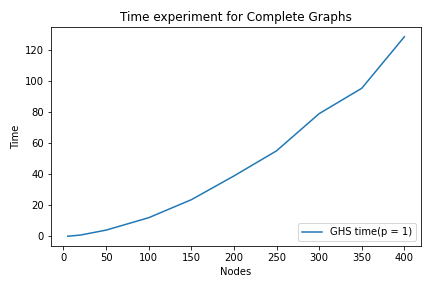
\includegraphics{time}
	
	\subsection{Complexity Analysis}
	
	Plots for the results on number of messages as given in the previous section are as follows : 
	
	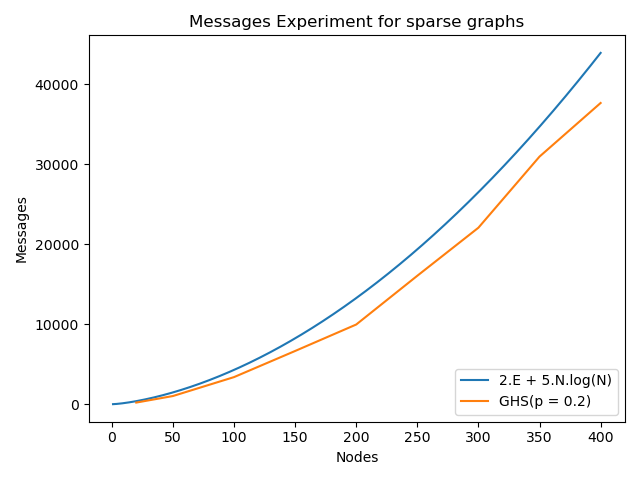
\includegraphics[width = 0.7 \textwidth]{sparse}
	
	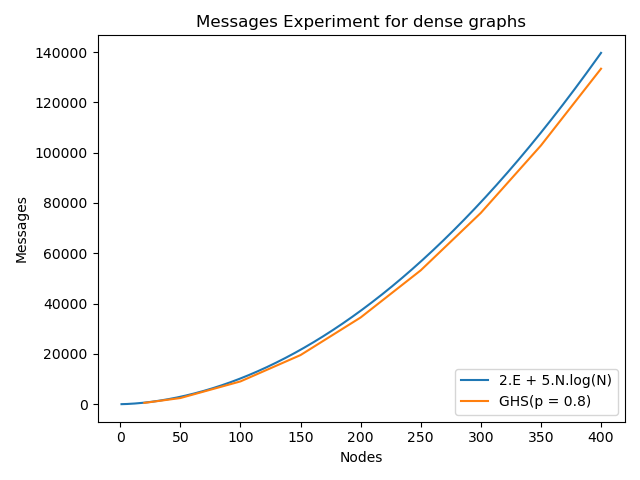
\includegraphics[width = 0.7 \textwidth]{dense}
	
	\newpage 
	
	In these plots 
	\begin{itemize}
		\item The blue line represents the function : $2 \cdot E + 5 \cdot N \cdot \log_2(N)$ with $N$ = number of nodes, $E$ = number of Edges.
		\item Here roughly $E = {N \choose 2} \cdot P$, where P is the probability that there is an edge between any two given nodes.
		\item The orange line represents the number of messages sent by all the nodes in our implementation.
	\end{itemize} 

	{\bf Analysis } :
	\begin{itemize}
		\item Clearly the orange line lies below the blue line for both, spare and dense graphs.
		\item As probability increases, the gap between the two lines decreases. 
		\item The blue line is therefore a tight upper bound on the total number of messages in GHS Algorithm. 
		\item Therefore the total number of messages sent in the GHS Algorithm grows as $2 \cdot E + 5 \cdot N \cdot \log_2(N)$
	\end{itemize}
\end{document}
